\documentclass{article}

% Include necessary packages
\usepackage{amsmath} % for mathematical notation
\usepackage{amssymb} % for mathematical symbols
\usepackage{algorithm} % for typesetting algorithms
\usepackage{algorithmic} % for typesetting algorithms
\usepackage{listings} % for typesetting code
\usepackage{color} % for syntax highlighting
\usepackage{geometry} % for adjusting margins
\usepackage{graphicx}

\graphicspath{ {./images/} }

\geometry{margin=1in}

\title{COMP3311 Notes}
\begin{document}

\section*{\huge COMP3311 Notes}
~\\
\section{Week 1}
\subsection{Intro to Database Systems}
~\\
\textbf{What technologies are used?} \\
- PostgreSQL (v13) \\
- SQLite (v3.x) \\
- Python (v3.9+) \\
- psycopg2 (v2.8+) 
\\\\
\textbf{Aims of data modelling:} \\
- Describe what \emph{information} is contained in the database \\
- Describe \emph{relationships} between data items \\
- Describe \emph{constraints} on data
\subsection{Entity-Relationship Data Modelling}
\textbf{Intro to ER} \\
ER has three major modelling constructs: \\\\
- \textbf{attribute:} \emph{data item} describing a property of interest \\
- \textbf{entity:} collection of attributes describing \emph{object of interest} \\
- \textbf{relationship:} \emph{association} between entities (objects) \\
\\\\
\textbf{ER Diagrams} \\
\emph{ER diagrams} are a graphical tool for data modelling consisting of:\\\\
- a collection of \emph{entity set} definitions \\
- a collection of \emph{relationship set} definitions \\
- \emph{attributes} associated with entity and relationship sets \\
- connections between entity and relationship sets \\\\
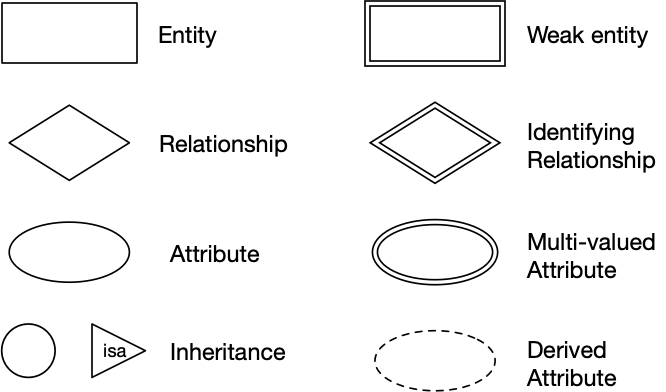
\includegraphics[scale=0.4]{ER_symbols} \\
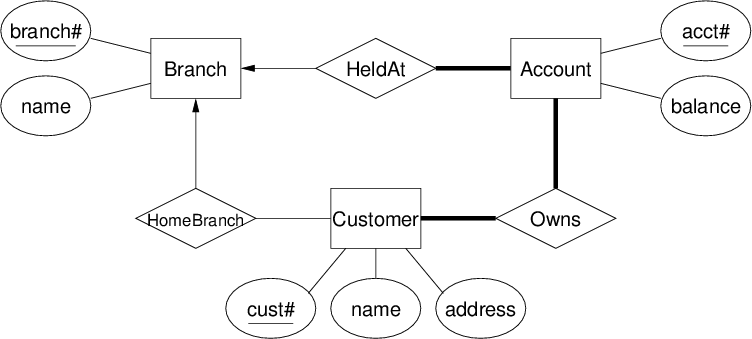
\includegraphics[scale=0.4]{ER_example}
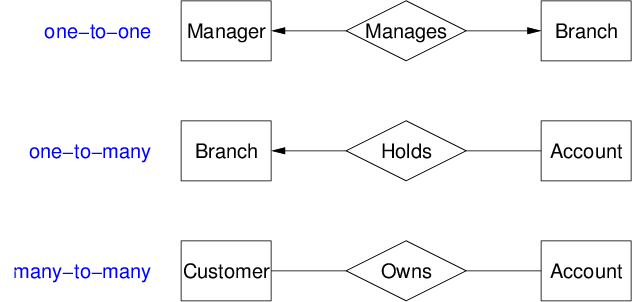
\includegraphics[scale=0.4]{ER_relationships}
\\\\
\textbf{ER Class Hierarchies} \\
ER implements \emph{super} and {sub} class hierarchies.
\\\\
- Superclasses have common properties with all entities in the hierarchy \\
- Subclasses are derived from the superclass and can be thought of as a child within the hierarchy
\subsection{Relational Modelling}
\textbf{Intro to RM} \\
World is modelled via tuples, relations and constraints. \\\\
\emph{Tuples} are collections of values \\
- e.g (123456, John Smith, 75.2) \\\\
\emph{Relations} are sets of tuples \\
- e.g { (1,2,3), (3,2,1) } \\\\
\emph{Constraints} are logical statements on valid data \\
- e.g. zID is unique  and  0 $\leq$ WAM $\leq$ 100 \\
\\
Types of Constraints: \\
- \emph{unique} = value of attribute is unique in relation \\
- \emph{key} = chosen unique attribute to distinguish tuples \\
- \emph{domain} = type of attribute, restrictions within type \\
- \emph{referential integrity} = foreign key
\end{document}